\documentclass[aspectratio=169,t,xcolor=table]{beamer}
\usepackage[utf8]{inputenc}

\usepackage{booktabs} 
\usepackage{subcaption}
\usepackage{epigraph}
\usepackage[outercaption]{sidecap}    
\usepackage{tikz}


\usetheme{Ufg}

%-------------------------------------theorems--------------
\newtheorem{conj}{Conjetura}
\newtheorem{defi}{Definition}
\newtheorem{teo}{Teorema}
\newtheorem{lema}{Lema}
\newtheorem{prop}{Proposição}
\newtheorem{cor}{Corolário}
\newtheorem{ex}{Example}
\newtheorem{exer}{Exercício}

\setbeamertemplate{theorems}[numbered]
\setbeamertemplate{caption}[numbered]

%-------------------------------------------------------------%
%----------------------- Primary Definitions -----------------%

\definecolor{color1}{RGB}{0,0,90} % Color of the article title and sections
\definecolor{color2}{RGB}{0,20,20} % Color of the boxes behind the abstract and headings
\definecolor{keys1}{rgb}{0.0, 0.29, 0.33}
\definecolor{keys2}{rgb}{0.25, 0.7, 0.55}
\definecolor{keys3}{rgb}{0.1, 0.3, 0.4}
\definecolor{keys4}{rgb}{0.21, 0.46, 0.53}
\definecolor{strings}{rgb}{0.0, 0.47, 0.44}
\definecolor{comments}{rgb}{0.4, 0.4, 0.5}
\definecolor{terminaltext}{rgb}{1,1,1}
\definecolor{terminalbackground}{rgb}{0.2,0.2,0.25}

\usepackage{listings}

\lstset{
  xleftmargin=8pt,
  xrightmargin=0pt,
  framexleftmargin=0pt,
  framexrightmargin=0pt,
  basicstyle={\fontsize{8pt}{10pt}\ttfamily},
  columns=flexible,
  keepspaces=false,
  showstringspaces=false,
  commentstyle= \color{comments},
  stringstyle= \color{strings},
  breaklines=false,
  postbreak=\mbox{$\hookrightarrow$\space}
}

\lstdefinelanguage{Terminal}{
  framexleftmargin=3pt,
  framexrightmargin=3pt,
  framextopmargin=3pt,
  framexbottommargin=3pt,
  backgroundcolor=\color{terminalbackground},
  basicstyle={\fontsize{8pt}{10pt}\ttfamily\color{terminaltext}},
}

%%% Bibliography
\usepackage[style=numeric,backend=biber]{biblatex}
\addbibresource{thud.bib}


% This command set the default Color, is also possible to choose a custom color
\setPrimaryColor{UFGBlue} 

% First one is logo in title slide (we recommend use a horizontal image), and second one is the logo used in the remaining slides (we recommend use a square image)
\setLogos{lib/logos/infw.png}{lib/logos/infw2.png} 

% -------------------------------------- Title Slide Information
\begin{document}
\title[Inf UFG]{MONID}
\subtitle{A Temporal Logic Based Framework for Intrusion Detection}

\author{Zanolin Lorenzo\inst{1}}

\institute[UFG] % (optional)
{
  \inst{1}%
  DMIF\\
  University of Udine
}
\date{September 2023}
%-----------------------The next statement creates the title page.
\frame[noframenumbering]{\titlepage}

%------------------------------------------------Slide 1
\setLayout{vertical} % This command define the layout. 'vertical' can be replace with 'horizontal', 'blank, 'mainpoint', 'titlepage'

\begin{frame}
    \frametitle{Table of Contents}
    \tableofcontents
\end{frame}
%---------------------------------------------------------

\section{Introduction}

\setLayout{mainpoint}
\setBGColor{DarkPurple}
\begin{frame}{}
    \frametitle{Introduction}
\end{frame}
\setLayout{vertical}

\begin{frame}
    \frametitle{Intrusion Detection}
    \textit{Intrusion detection} means maintaining constant surveillance on a system in order to detect any misuse of these weak areas as soon as feasible so that they can be repaired.\\
    There are three approaches:
    \begin{itemize}
        \item \textit{signature-based}: aims to identify patterns and match them with known signs of intrusions;
        \item \textit{anomaly-based}: can identify new attacks when it detects behavior that differs significantly from previously learned normal behavior;
        \item \textit{hybrid}: combines the best of both worlds by looking at patterns and one-off events.
    \end{itemize}
    \vspace{5mm}
    We will present MONID which is a \textit{signature-based} intrusion detector.
\end{frame}

\begin{frame}
    \frametitle{What is MONID?}
    MONID is a prototype which can detect intrusions on a system and operates in both online and offline modes.\\
    \vspace{5mm}
    In order:
    \begin{enumerate}
        \item we will use the logic \textbf{EAGLE} to define intrusion patterns using temporal logic formula $\varphi$; in this case the monitored formula will be $\psi=\square (\neg\varphi)$.
        \item MONID will create a stream of events $\sigma=\alpha_{1},\alpha_{2},\ldots$ obtained from a merge of the logs by ascending time order;
        \item a monitor will processes each event $\alpha_i$ as it happens and updates the monitored formula $\psi$ to store a relevant summary;
        \item an intrusion alarm is triggered if, for any reason, $\alpha_{1},\alpha_{2} \ldots\not\models\psi$.
    \end{enumerate}
    
\end{frame}

\begin{frame}
    \frametitle{What is MONID? (cont'd)}
    The architecture is the following.\\
    \vspace{2.5mm}
    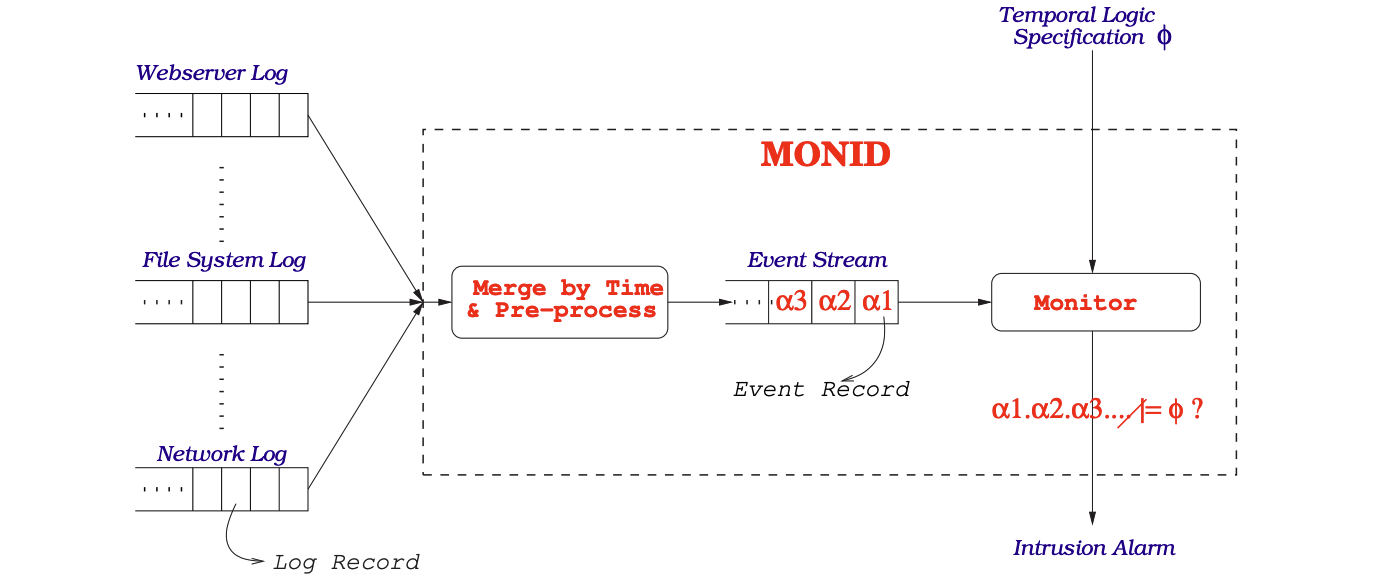
\includegraphics[scale=0.25]{images/monid.png}
    \vspace{2.5mm}\\
    Now, let us start from the basics of EAGLE.
\end{frame}





\begin{frame}[allowframebreaks]{References}
    \nocite{*} 
    \printbibliography
\end{frame}

\setLayout{mainpoint}
\setBGColor{DarkGray}
\begin{frame}{}
    \frametitle{Thanks for the attention}
\end{frame}
\setLayout{vertical}

\end{document}